
\chapter{Collection data types}

\section{Sequence types}

\begin{tcolorbox}
  A \keyword{sequence} type is one that support:
  \begin{itemize}
  \item the membership operator (\verb|in|)
  \item the size function (\verb|len()|) 
  \item slices ([]) 
  \item and is iterable.
  \end{itemize}
  Python provides five built-in sequence types:
  \begin{itemize}
  \item bytearray
  \item bytes
  \item list
  \item str
  \item tuple
  \end{itemize}
  When iterated, all of these sequences provide their items in order.
\end{tcolorbox}



\subsection{Tuples}

Tuples are immutable.
Tuples are able to hold any items of any data type, including collection types such as tuples and lists, since what they really hold are object references.

Tuples provide just two methods, \verb|t.count(x)| and \verb|t.index(x)|.

\begin{tcolorbox}
  tuple coding style:
  omit parentheses:
  \begin{itemize}
  \item tuples on the left-hand size of a binary operator
  \item on the right-hand size of a unary statement
  \end{itemize}
  other cases with parentheses.

  \begin{lstlisting}

a, b = (1, 2)  # left of binary operator
del a, b       # right of unary operator
  \end{lstlisting}

\end{tcolorbox}


When we have a sequences on the right-hand side of an assignment, and
we have a tuple on the left-hand side,
we say that the right-hand side has been \keyword{unpacked}.
Sequence unpacking can be used to swap values, for example:
\begin{lstlisting}

a, b = (b, a) # or a, b = b, a
# the parentheses here are for code style

for x, y in ((3, 4), (5, 12), (28, -45):
    print(math.hypot(x, y))
\end{lstlisting}



\subsection{Named tuples}


A named tuple behaves just like a plain tuple, and has the same performance characteristics.
What it adds is the ability to refer to items in the tuple by name as well as by index position.


\begin{lstlisting}

import collections

Fullname = collections.namedtuple('Fullname',
                                  'firstname middlename lastname')
persons = []
persons.append(Fullname('Mike', 'Ming', 'Chyson'))
persons.append(Fullname('Alfred', 'Bernhard', 'Nobel'))
for person in persons:
    print('{firstname} {middlename} {lastname}'.format(**person._asdict()))

\end{lstlisting}



\subsection{Lists}

List are mutable.
Since all the items in a list are really object references, lists can hold items of any data type, including collection types such as lists and tuples.


Although we can use the slice operator to access items in a list, in some situations we want to take two or more pieces of a list in one go.
This can be done by sequence unpacking.
Any iterable (lists, tuples, etc.) can be unpacked using the sequence unpacking operator, an asterisk or star (*).
When used with two or more variables on the left-hand side of an assignment, one of which is preceded by *, items are assigned to the variables, with all those left over assigned to the starred variable.
Here are some examples:

\begin{lstlisting}

>>> a = list(range(10))
>>> first, *last = a
>>> print(first, last)
0 [1, 2, 3, 4, 5, 6, 7, 8, 9]
>>> 
>>> first, *middle, last = a
>>> print(first, middle, last)
0 [1, 2, 3, 4, 5, 6, 7, 8] 9
>>> 
>>> *first, last = a
>>> print(first, last)
[0, 1, 2, 3, 4, 5, 6, 7, 8] 9
\end{lstlisting}



List methods:
\begin{description}
\item[list.append(x)] 
\item[list.count(x)] 
\item[list.extend(m)] 
\item[list += m] 
\item[list.index(x, start, end)] 
\item[list.insert(i, x)] 
\item[list.pop()] Returns and removes the rightmost item of list
\item[list.pop(i)] 
\item[list.remove(x)] Removes the leftmost occurrence of item x from list
\item[list.reverse()] Reverses list in-place
\item[list.sort(...)] Sorts list in-place
\end{description}


Individual items can be replaced in a list by assigning to a particular index position.
Entire slices can be replaced by assigning an iterable to a slice.
The slice and the iterable don't have to be the same length.
In all cases, the slice's items are removed the the iterable's items are inserted.

\begin{lstlisting}

>>> nums = [0, 1, 2, 3, 4, 5, 6]
>>> nums[0] = 100
>>> nums
[100, 1, 2, 3, 4, 5, 6]
>>> nums[2:2] = [200]    # same to nums.insert(2, 200)
>>> nums
[100, 1, 200, 2, 3, 4, 5, 6]
>>> nums[2:4] = [10, 11, 12, 13, 14]
>>> nums
[100, 1, 10, 11, 12, 13, 14, 3, 4, 5, 6]
\end{lstlisting}


In lists, striding allows us to access every n-th item which can often be useful.
For example:
\begin{lstlisting}

>>> x = list(range(1, 11))
>>> x
[1, 2, 3, 4, 5, 6, 7, 8, 9, 10]
>>> x[1::2] = [0] * len(x[1::2])
>>> x
[1, 0, 3, 0, 5, 0, 7, 0, 9, 0]
\end{lstlisting}


\begin{lstlisting}
>>> x = list(range(-5, 5))
>>> x
[-5, -4, -3, -2, -1, 0, 1, 2, 3, 4]
>>> x.sort(key=lambda x: x**2)
>>> x
[0, -1, 1, -2, 2, -3, 3, -4, 4, -5]
\end{lstlisting}




For inserting items, lists perform best when items are added or removed at the end (\verb|list.append(), list.pop()|).
The worst performance occurs when we search for items in a list, for example, using \verb|list.remove()| or \verb|list.index()|, or using \verb|in| for membership testing.
If fast searching or membership testing is required, a \verb|set| or a \verb|dict| may be a more suitable collection choice.
Alternatively, lists can provide fast searching if they are kept in order by sorting them and using a binary search (provided by the \verb|bisect| module), to find items. 


\subsection{List comprehensions}

A \keyword{list comprehension} is an expression and a loop with optional condition enclosed in brackets where the loop is used to generate items for the list, and where the condition can filter out unwanted items.

\begin{verbatim}
[expression for item in iterable]
[expression for item in iterable if condition]
\end{verbatim}


\begin{lstlisting}
  leaps = [y for y in range(1900, 1940)
           if (y % 4) == 0 and y % 100 != 0) or (y % 400 == 0)]
\end{lstlisting}


If the generated list is very large, it may be more efficient to generate each item as it is needed rather than produce the whole list at once.
This can be achieved by using a generator rather than a list comprehension. 



\section{Set types}

\begin{tcolorbox}
A \keyword{set} is a collection data type that supports:
\begin{itemize}
\item the membership operator(\verb|in|),
\item the size function (\verb|len()|),
\item and is iterable.
\end{itemize}
Python provides two built-in set types:
\begin{itemize}
\item the mutable \verb|set| type
\item the immutable \verb|frozenset|
\end{itemize}
When iterated, set types provide their items in an arbitrary order.
\end{tcolorbox}



Only \keyword{hashable} objects may be added to a set.
Hashable objects are objects which have a \verb|__hash__()| special method whose return value is always the same thoughout the ojbect's lifetime, and which can be compared for equality using the \verb|__eq__()| special method.
(Special mehtods are methods whose name begins and ends with two underscores)



\subsection{Sets}

A \keyword{set} is an unordered collection of zero or more object references that refer to hashable objects.
Sets are mutable.
Sets always contain unique items --- adding duplicate items is safe but pointless.


\begin{figure}[!ht]
  \centering
  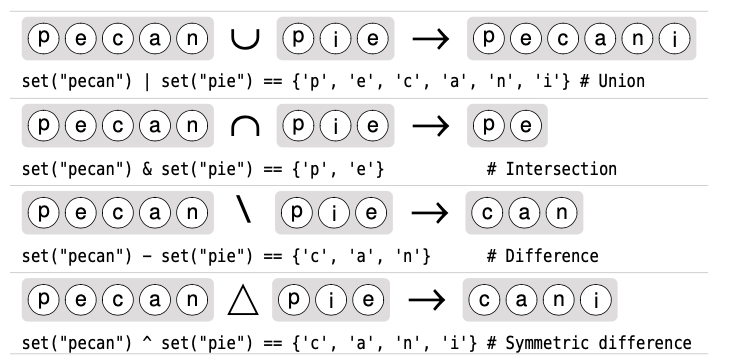
\includegraphics[width=\textwidth]{pics/standard-set-operators}
  \caption{Standard set operators}
  \label{fig:standard-set-operators}
\end{figure}


Set methods:
\begin{description}
\item[s.add(x)] 
\item[s.clear()] 
\item[s.copy()] 
\item[s.difference(t)] Same to s - t
\item[s.difference\_{}update(t)] Same to s -= t
\item[s.discard] Removes item x from set s if it is in s
\item[s.remove()] Removes item x from set s, or raises a KeyError exception if x is not in s
\item[s.intersection(t)] Same to s \& t
\item[s.intersection\_{}update(t)] Same to s \&= t
\item[s.isdisjoint(t)] Returns True if sets s and t have no items in common
\item[s.issubset(t)] Same to s <= t
\item[s.issuperset(t)] Same to s >= t
\item[s.pop()] Returns and remove a random item from set s, or raises a KeyError exception if s is empty
\item[s.symmetric\_{}difference(t)] Same to s \^{} t
\item[s.symmetric\_{}difference\_{}update(t)] Same to s\^{}= t
\item[s.union(t)] Same to s | t
\end{description}


Sets are used used for fast membership test and removring duplicated items.


\subsection{Set comprehensions}

\begin{verbatim}
{expression for item in iterable}
{expression for item in iterable if condition}
\end{verbatim}

\subsection{Frozen sets}

A frozen set is a set that, once created, cannot be changed.
Since frozen set are immutable, sets and frozen sets can contain frozen sets.



\section{Mapping types}

\begin{tcolorbox}
A \keyword{mapping} type is one that supports:
\begin{itemize}
\item the membership operator (in)
\item the size function (len())
\item is iterable 
\end{itemize}

Mappings are collection of key-value items and provide methods for accessing items and their keys and values.
\end{tcolorbox}

When iterated, unordered mapping types provide their items in an arbitrary order.


There are one built-in mapping types and two standard library's mapping types:
\begin{itemize}
\item dict
\item collections.defaultdict
\item collections.OrderedDict
\end{itemize}



\subsection{Dictionaries}

A \verb|dict| is an unordered collection of zero or more key–value pairs whose keys are object references that refer to hashable objects, and whose values are object references referring to objects of any type.
Dictionaries are mutable.

\begin{lstlisting}
>>> d = dict()
>>> d
{}
>>> d = {}
>>> d
{}
>>> d = {"hello": 1, "world": 2}
>>> d
{'hello': 1, 'world': 2}
>>> d = dict(hello=1, world=2)
>>> d
{'hello': 1, 'world': 2}
>>> d = dict([("hello", 1), ("world", 2)])
>>> d
{'hello': 1, 'world': 2}  
\end{lstlisting}



Dictionary methods:
\begin{description}
\item[d.clear()] 
\item[d.copy()] 
\item[d.fromkeys(s, v)] Returns a dict whose keys are the items in sequence s and whose values are None or v if v is given
\item[d.get(k)] Returns key k's associated value or None if k isn't in dict d
\item[d.get(k, v)] Returns key k's associated value, or v if k isn't in dict d
\item[d.items()] 
\item[d.keys()] 
\item[d.values()] 
\item[d.pop(k)] 
\item[d.pop(k, v)] 
\item[d.popitem()] Returns and removes an arbitrary (key, value) pair from dict d
\item[d.setdefault(k, v)] The same as the dict.get() method, except that if the key is not indict d,a new item is inserted with the key k, and with a value of None or of v if v is given
\item[d.update(a)] Adds every (key, value) pair from a that isn’t in dict d to d, and for every key that is in both d and a, replaces the corresponding value in d with the one in a --— a can be a dictionary, an iterable of (key, value) pairs, or keyword arguments
\end{description}



The \verb|dict.items()|, \verb|dict.keys()|, and \verb|dict.values()| methods all return dictionary views.
A dictionary view is effectively a read-only iterable object that appears to hold the dictionary’s items or keys or values, depending on the view we have asked for.


In general, we can simply treat views as iterables.
However, two things make a view different from a normal iterable.
One is that if the dictionary the view refers to is changed, the view reflects the change.
The other is that key and item views support some set-like operations.
Given dictionary view \verb|v| and \verb|set| or dictionary view \verb|x|, the supported operations are:
\begin{verbatim}
v & x  # intersection
v | x  # union
v - x  # difference
v ^ x  # symmetric difference
\end{verbatim}



\begin{lstlisting}
>>> d = {}.fromkeys("abcd", 3)
>>> d
{'a': 3, 'b': 3, 'c': 3, 'd': 3}
>>> s = set("abc")
>>> s
{'a', 'c', 'b'}
>>> d.keys() & s
{'a', 'c', 'b'}
>>> 
>>> d
{'a': 3, 'b': 3, 'c': 3, 'd': 3}
>>> d.setdefault('a')
3
>>> d
{'a': 3, 'b': 3, 'c': 3, 'd': 3}
>>> d.setdefault('z', 100)
100
>>> d
{'a': 3, 'b': 3, 'c': 3, 'd': 3, 'z': 100}  
  
\end{lstlisting}




\subsection{Dictionary comprehensions}

\begin{lstlisting}
{keyexpression: valueexpression for key, value in iterable}
{keyexpression: valueexpression for key, value in iterable if condition}
\end{lstlisting}


\begin{lstlisting}
import os

# filename: filesize
d = {name: os.path.getsize(name) for name in os.listdir('.') if os.path.isfile(name)}
print(d)

# revert dict
inserted_d = {v: k for k, v in d.items()}
print(inserted_d)  
\end{lstlisting}


\subsection{Default dictionaries}

Default dictionaries are dictionaries --- they have all the operators and methods that dictionaries provide.
What makes default dictionaries different from plain dictionaries is the way they handle missing keys.



When a default dictionary is created, we can pass in a \keyword{factory function}.
A factory function is a function that, when called, returns an object of a particular type.
All of Python’s built-in data types can be used as factory functions.
The factory function passed to a default dictionary is used to create default values for missing keys.


\begin{tcolorbox}
  Note that the \keyword{name} of a function is an object reference to the function --- so when we want to pass functions as parameters, we just pass the name.
  When we use a function with parentheses, the parentheses tell Python that the function should be called.
\end{tcolorbox}

\begin{lstlisting}
>>> words = collections.defaultdict(int)
>>> words
defaultdict(<class 'int'>, {})
>>> words['hello'] += 1
>>> words
defaultdict(<class 'int'>, {'hello': 1})
>>> words['hello'] += 1
>>> words
defaultdict(<class 'int'>, {'hello': 2})
>>> 
>>> de = collections.defaultdict(lambda : "Thanks to ")
>>> de
defaultdict(<function <lambda> at 0x7fa999a75a60>, {})
>>> de['Mike'] += 'Mike'
>>> de
defaultdict(<function <lambda> at 0x7fa999a75a60>, {'Mike': 'Thanks to Mike'})  
\end{lstlisting}


\subsection{Ordered dictionaries}
The ordered dictionaries type is \verb|collections.OrderedDict|
Ordered dictionaries store their items in the order in which they were inserted.
If we change an item's value, the order is not changed.


\begin{lstlisting}
d = collections.OrderedDict([('z', -4), ('e', 19), ('k', 7)])
for k in d:
    print(k, d[k])
    
tasks = collections.OrderedDict()
tasks[8031] = "Backup"
tasks[4027] = "Scan Email"
tasks[5733] = "Build System"
for k in tasks:
    print(k, tasks[k])  
\end{lstlisting}


If we want to move an item to the end, we must delete it and then reinsert it.
We can also call \verb|popitem()| to remove and return the last key–value item in the ordered dictionary; or we can call
\verb|popitem(last=False)|, in which case the first item will be removed and returned.



\section{Iterating and copying collections}

\subsection{Iterators and iterable operations and functions}

An \keyword{iterable} data type is one that can return each of its items one at a time.
Any object that has an \verb|__iter__()| method, or any sequence (i.e. an object that has a \verb|__getitem__()| method taking integer arguments starting from 0) is an iterable and can be provide an \keyword{iterator}.
An iterator is an object that provides a \verb|__next__()| method which returns each successive item in turn, and raises a \verb|StopIteration| exception when there are no more items.


The operators and functions that can be used with iterables:
\begin{description}
\item[s + t] Returns a sequence that is the concatenation of sequences s and t
\item[s * t] Returns a sequences that is int n concatenation of sequences s
\item[x in i] Returns True if item x is in iterable i
\item[all(i)] Returns True if every item in iterable i evalueates to True
\item[any(i)] Returns True if any item in iterable i evalueates to True
\item[enumerate(i, start)] Normally used in for ... in loops to provide a sequence of (index, item) tuples with indexes starting at 0 or start
\item[len(x)] 
\item[max(i, key)] Returns the biggest item in iterable i or the item with the biggest key(item) value if a key function is given
\item[min(i, key)] Returns the smallest item in iterable i or the item with the smallest key(item) value if a key function is given
\item[range(start, stop, step)] Returns an integer iterator.
\item[reversed(i)] Returns an iterator that returns the items from iterator i in reverse order
\item[sorted(i, key, reverse)] Return a list of the items from iterator i in sorted order; key is used to provide DSU (Decorate, Sort, Undecorate) sorting. If reverse is True the sorting is done in reverse order.
\item[sum(i, start)] Returns the sum of the items in iterable i plus start (which defaults to 0)
\item[zip(i1, ..., iN)] Returns an iterator of tuples using the iterators i1 to iN
\end{description}


The order in which items are returned depends on the underlying iterable.
In the case of lists and tuples, items are normally returned in sequential order starting from the first item (index position 0), but some iterators return the items in an arbitrary order --- for example, dictionary and set iterators.


The built-in \verb|iter()| function has two quite different behaviors.
\begin{itemize}
\item When given a collection data type or a sequence it returns an iterator for the oject it is passed --- or raise a \verb|TypeError| if the object cannot be iterable.
\item When given a callable (a function or method) and a sentinel value, the function passed in is called once at each iteration, returning teh function'sreturn value each time, or raising a \verb|StopIteration| exception if the return value equals the sentinel.
\end{itemize}




When we use a \verb|for item in iterable| loop, Python in effect calls \verb|iter(iterable)| to get an iterator.
This iterator's \verb|__next__()| method is then called at each loop iteration to get the next item, and when the \verb|StopIteration| exception is raised, it is caughted and the loop is terminated.



\begin{lstlisting}
# manner 1
product = 1
for i in [1, 2, 4, 8]:
    product *= i
print(product)


# manner 2
product = 1
i = iter([1, 2, 4, 8])
while True:
    try:
        product *= i
    except StopIteration:
        break
print(product)  
\end{lstlisting}



Any (finite) iterable, i, can be converted into a tuple by calling \verb|tuple(i)|, or can be converted into a list by calling \verb|list(i)|.




\begin{lstlisting}
>>> x = []
>>> for t in zip(range(-10, 0, 1), range(0, 10, 2), range(1, 10, 2)):
...     x += t
... 
>>> x
[-10, 0, 1, -9, 2, 3, -8, 4, 5, -7, 6, 7, -6, 8, 9]
>>> sorted(x)
[-10, -9, -8, -7, -6, 0, 1, 2, 3, 4, 5, 6, 7, 8, 9]
>>> sorted(x, reverse=True)
[9, 8, 7, 6, 5, 4, 3, 2, 1, 0, -6, -7, -8, -9, -10]
>>> sorted(x, key=abs)
[0, 1, 2, 3, 4, 5, 6, -6, -7, 7, -8, 8, -9, 9, -10]  
\end{lstlisting}


\begin{tcolorbox}
  A function's name is an object reference to the function;
  it is the parentheses that follow the name that tell Python to call the function.
\end{tcolorbox}


Python's sort algorithm is an adaptive stable mergesort that is both fast and smart, and it is especially well optimized for partially sorted lists.
The ``adaptive'' part means that the sort algorithm adapts to circumstances --- for example, taking advantage of partially sorted data.
The ``stable'' part means that the items that sort equally are not moved in relation to each other.
When sorting collections of itegers, strings, or other simple types their ``less than'' operator (<) is used.
Python can sort collections that contain collections, working recursively to any depth.



Lists can be sorted in-place using the \verb|list.sort()| method, which takes the same optinal arguments as \verb|sorted()|.


\subsection{Copying collections}

Since Python uses \keyword{object references}, when we use the assignment operator (+), no copying takes place.
If the right-hand operand is a literal such as a string or a number, the left-hand operand is set to be an object reference that refers to the in-memory object that holds the literal’s value.
If the right-hand operand is an object reference, the left-hand operand is set to be an object reference that refers to the same object as the right-hand operand.
One consequence of this is that assignment is very efficient.



For sequences, when we take a slice, the slice is always an independent copy of the items copied.
For dictionaries and sets, copying can be achived using \verb|dict.copy()| and \verb|set.copy()|.
In addition, the \verb|copy| module provides the \verb|copy.copy()| function that returns a copy of the object it is given.
Another way to copy the built-in collection types is to use the type as a function with the collection to be copied as its argument.




\begin{tcolorbox}
  Note, thought, that all of these copying techniques are \keyword{shallow} --- that is, only object references are copied and not the object themselves.
  For immutable data types like numbers and strings this has the same effect as copying, but for mutable data types such as nested collections this means that the object they refer to are referred to both by the original collection and by the copied collection.


  \begin{lstlisting}
    print('{:.^50}'.format('print(x,y)'))
    x = [53, 68, ['A', 'B', 'C']]
    y = x[:]
    print(x, y, sep='\n')
    
    print('{:.^50}'.format('print(x,y)'))
    y[1] = 40
    x[2][0] = 'Q'
    print(x, y, sep='\n')

    """
    ....................print(x,y)....................
    [53, 68, ['A', 'B', 'C']]
    [53, 68, ['A', 'B', 'C']]
    ....................print(x,y)....................
    [53, 68, ['Q', 'B', 'C']]
    [53, 40, ['Q', 'B', 'C']]
    """
  \end{lstlisting}
\end{tcolorbox}



If we really need independent copies of arbitrarily nested collections, we can deep-copy:
\begin{lstlisting}
import copy

x = [53, 68, ['A', 'B', 'C']]
y = copy.deepcopy(x)
y[1] = 40
x[2][0] = 'Q'
print('{:.^50}'.format('print(x,y)'))
print(x, y, sep='\n')

"""
....................print(x,y)....................
[53, 68, ['Q', 'B', 'C']]
[53, 40, ['A', 'B', 'C']]
"""
\end{lstlisting}





